360 split with title

\documentclass[tikz,border=10pt]{standalone}
\usepackage{tikz}
\usetikzlibrary{angles,quotes,calc} % Add this for angle labels

\begin{document}

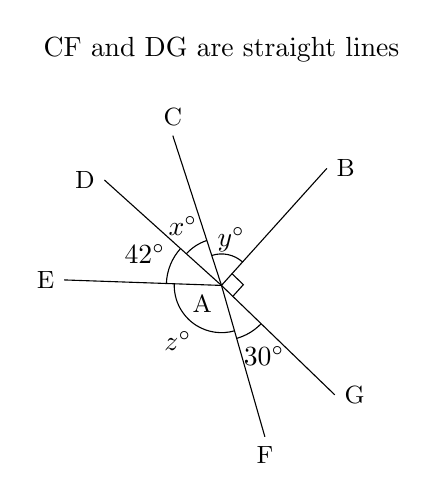
\begin{tikzpicture}[scale=1]

    % Define the points of the cube
    \coordinate (A) at (0,0);
    \coordinate (B) at ($(A)+(48:2cm)$); 
    \coordinate (C) at ($(A)+(108:2cm)$); 
    \coordinate (D) at ($(A)+(138:2cm)$); 
    \coordinate (E) at ($(A)+(178:2cm)$); 
    \coordinate (F) at ($(A)+(286:2cm)$); 
    \coordinate (G) at ($(A)+(316:2cm)$); 

    % Draw the right angle symbol at GAB
    \pic [draw, angle eccentricity=1, angle radius=0.2cm] {right angle = G--A--B};

    % Draw the visible edges of the cube
    \draw (A) -- (B);
    \draw (A) -- (C);
    \draw (A) -- (D);
    \draw (A) -- (E);
    \draw (A) -- (F);
    \draw (A) -- (G);
    
    % Draw the angle between lines
    \pic [draw, "$y^{\circ}$", angle eccentricity=1.5, angle radius=0.4cm] {angle = B--A--C};
    \pic [draw, "$x^{\circ}$", angle eccentricity=1.5, angle radius=0.6cm] {angle = C--A--D};
    \pic [draw, "$42^{\circ}$", angle eccentricity=1.5, angle radius=0.7cm] {angle = D--A--E};
    \pic [draw, "$z^{\circ}$", angle eccentricity=1.5, angle radius=0.6cm] {angle = E--A--F};
    \pic [draw, "$30^{\circ}$", angle eccentricity=1.5, angle radius=0.7cm] {angle = F--A--G};

    % Place the labels with smaller font size
    \node at (A) [below left,font=\small] {A};
    \node at (B) [right,font=\small] {B};
    \node at (C) [above,font=\small] {C};
    \node at (D) [left,font=\small] {D};
    \node at (E) [left,font=\small] {E};
    \node at (F) [below,font=\small] {F};
    \node at (G) [right,font=\small] {G};

    % Add labels at the top of the figure
    \node at (0, 3) {CF and DG are straight lines};
    
\end{tikzpicture}

\end{document}